\subsection{測定4:2台のレーザー間のうなりの測定}
偏光板あり,なしの状態でのうなりの周波数$F_1$と基本周波数$F_2$を表に示す.
\begin{table}[h]
\caption{うなりの周波数と基本周波数}
\label{tab:unari_kihon}
\centering
\begin{tabular}{ccc}
\hline
&うなりの周波数$F_1$ / $\times10^6\si{\hertz}$&基本周波数$F_2$ / $\times10^7\si{\hertz}$\\
\hline \hline
偏光板なし&$2.73$&$8.93$\\
偏光板あり&-&$4.00$\\
\hline
\end{tabular}
\end{table}
\begin{figure}[htbp]
  \begin{minipage}{0.5\hsize}
   \begin{center}
    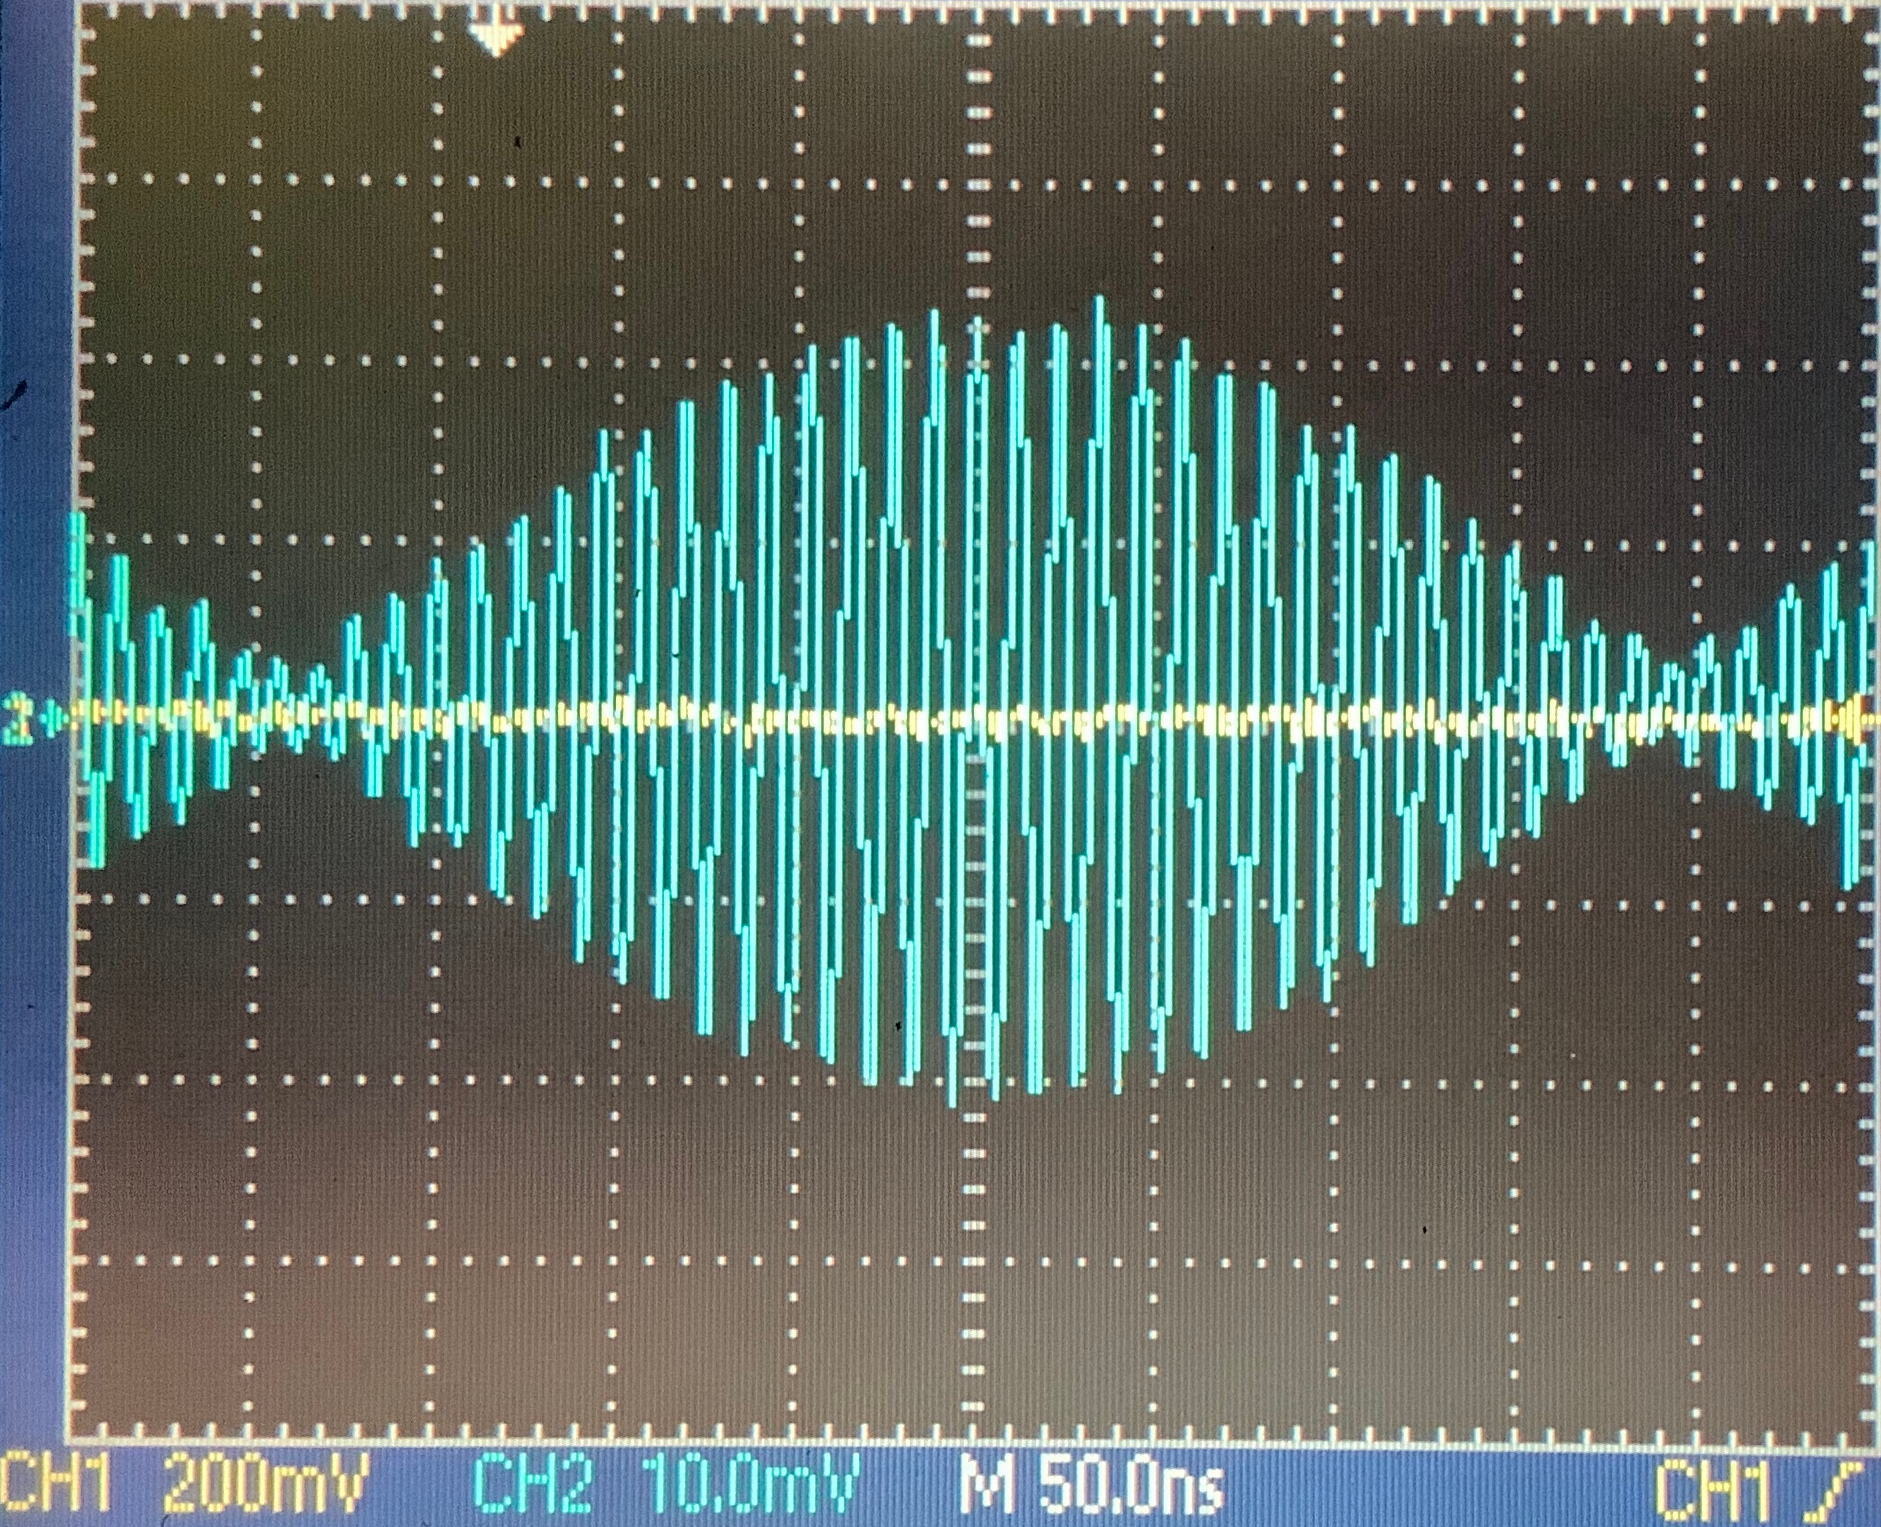
\includegraphics[width=60mm]{fig/fig7.JPG}
   \end{center}
   \caption{偏光板なし}
   \label{fig:no_polar}
  \end{minipage}
  \begin{minipage}{0.5\hsize}
   \begin{center}
    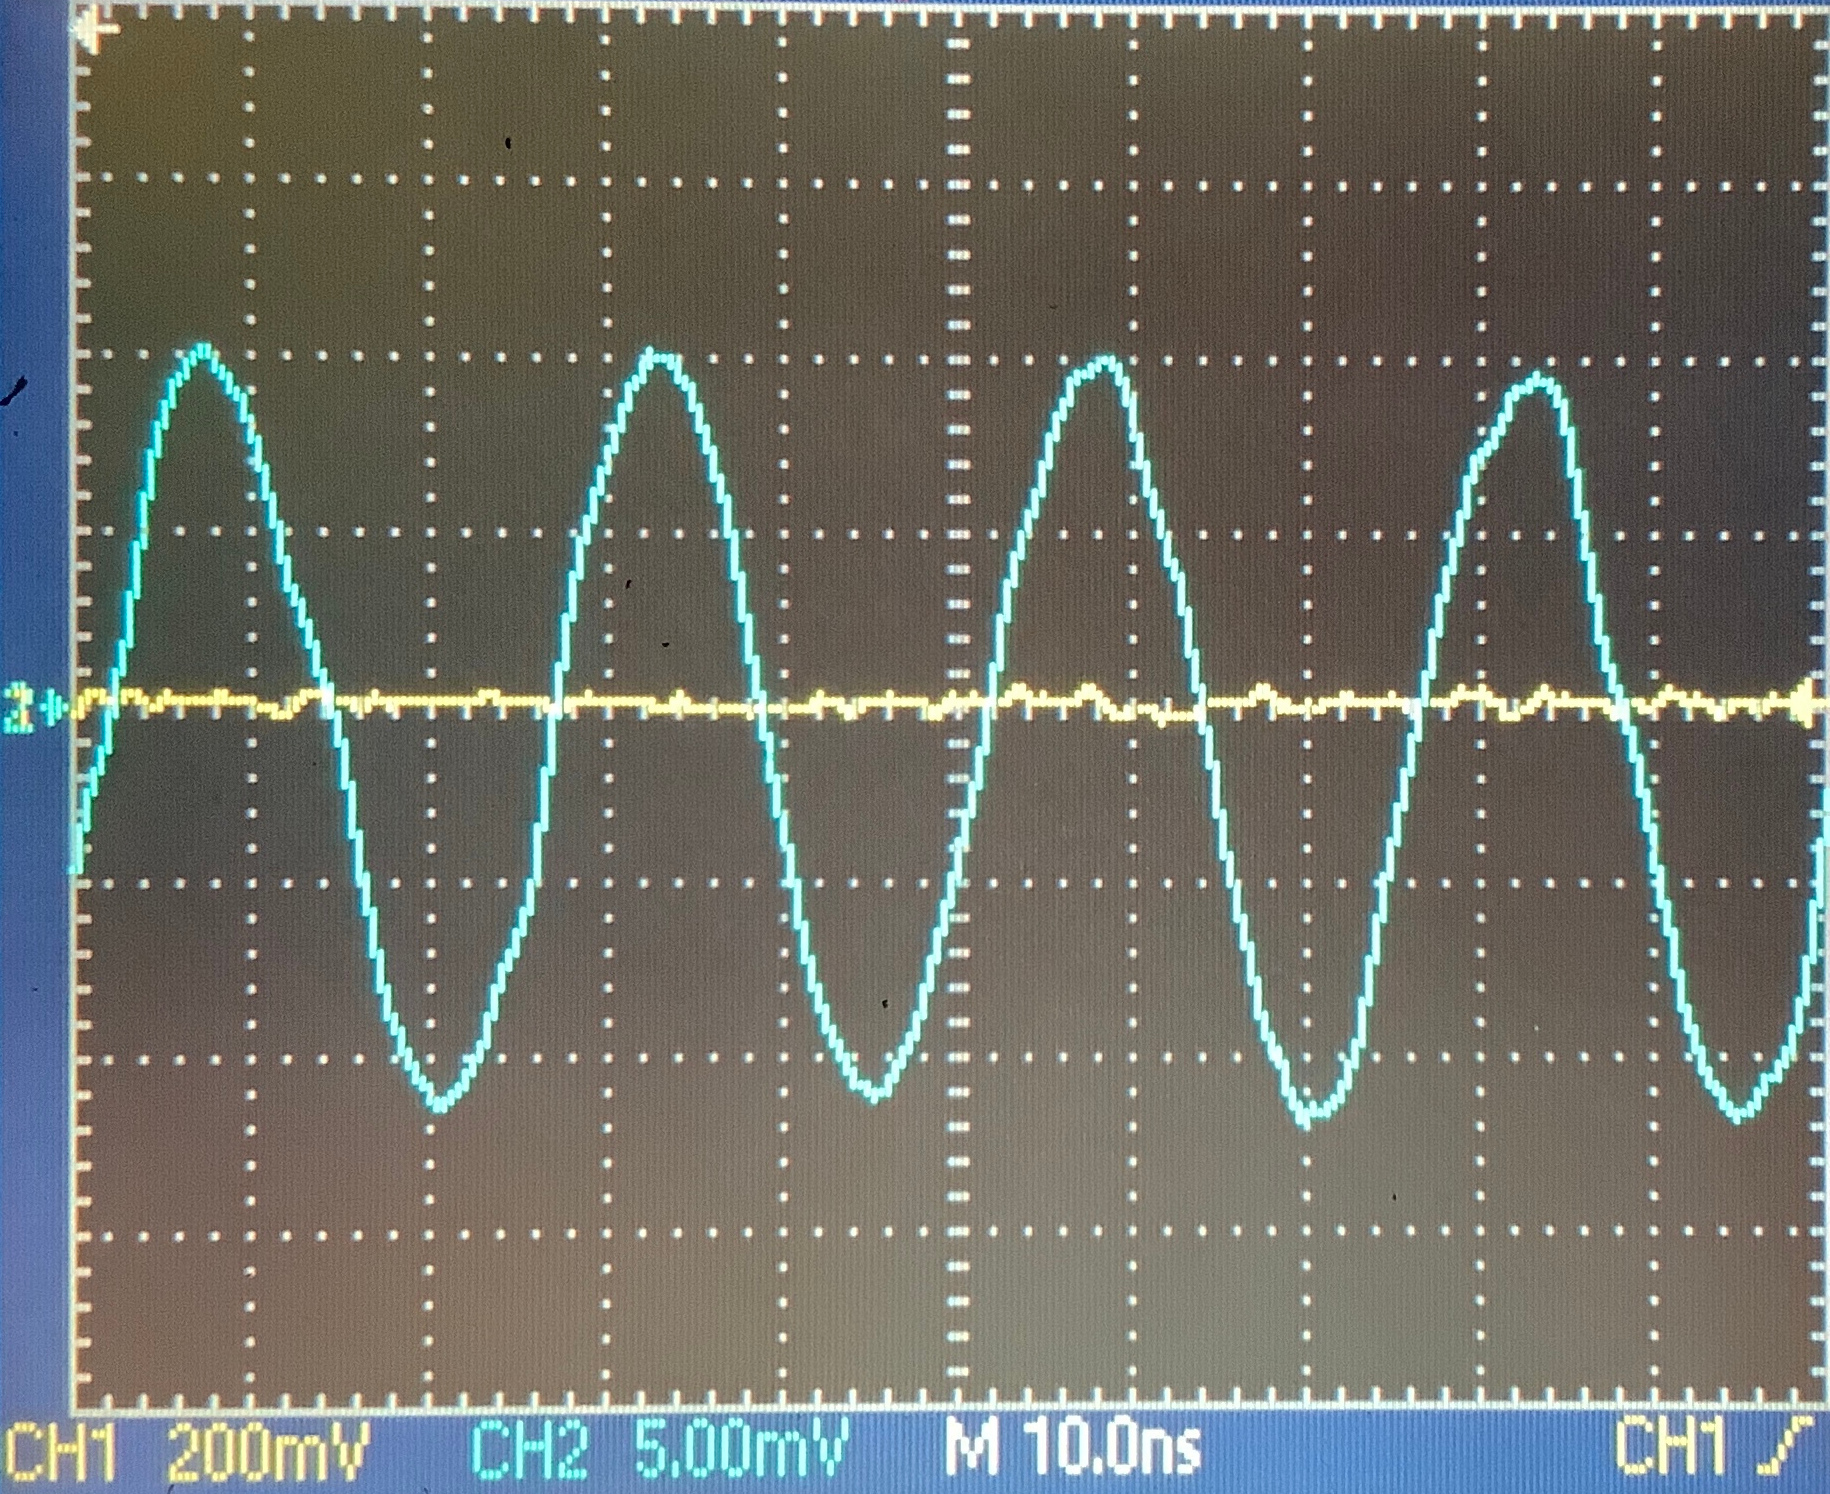
\includegraphics[width=60mm]{fig/fig8.JPG}
   \end{center}
   \caption{偏光板あり}
   \label{fig:polar}
  \end{minipage}
 \end{figure}